\documentclass[11pt,a4paper]{article}

\usepackage{graphicx}
\usepackage{listings}
\usepackage{url}
\title{Accessing GPIO pins of R-Pi}
\author{e-Yantra Team}
\date{\today}

\begin{document}
	\maketitle
	\newpage
	\tableofcontents
	\newpage
	\section{Objective}
	In this tutorial we will learn how to write simple programs to access GPIO pins in an R-Pi. 
	\section{Prerequisites}
	\begin{itemize}
		\item Python programming skills
		\item Basic terminal commands
	\end{itemize}
	\section{Hardware Requirement}
	\begin{enumerate}
		\item Raspberry Pi (I will be using Version 2 Model B)
		\item Power adapter
		\item Connecting wires
		\item LED
		\item Push button
		\item Resistor (330 ohms)
		\item Bread board
	\end{enumerate}
	\section{Software Requirement}
	\begin{enumerate}
		\item PyScripter (version 2.7 or above)
		\item Mobaxterm (for windows users)
	\end{enumerate}
	
	\newpage
	\section{Theory and Description}
	The Raspberry Pi 2 Model B is the second generation Raspberry Pi. Compared to the Raspberry Pi 1 it has:
	\begin{itemize}
	\item A 900MHz quad-core ARM Cortex-A7 CPU
	\item 1GB RAM
	\end{itemize}
	Like the (Pi 1) Model B+, it also has:
	\begin{itemize}
			\item 4 USB ports
			\item 40 GPIO pins
			\item Full HDMI port
			\item Ethernet port
			\item Combined 3.5mm audio jack and composite video
			\item Camera interface (CSI)
			\item Display interface (DSI)
			\item Micro SD card slot
			\item VideoCore IV 3D graphics core
			\item Because it has an ARMv7 processor, it can run the full range of ARM GNU/Linux distributions, including Snappy Ubuntu Core, as well as Microsoft Windows 10. [2]
	\end{itemize}
	
	\textbf{Expansion Header}
	
	The Raspberry Pi 2 Model B board contains a single 40-pin expansion header labelled as 'J8' providing access to 26 GPIO pins.
	(Pins 1, 2, 39 and 40 are also labelled below.)
			\begin{figure}[h!]
				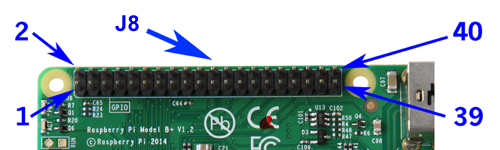
\includegraphics[scale=0.7]{j8h.png}
				\centering
				\caption{[3]}
			\end{figure} 
	
	\newpage
	The diagram below illustrates the pin out diagram of Raspberry Pi 2:
	\begin{figure}[h!]
		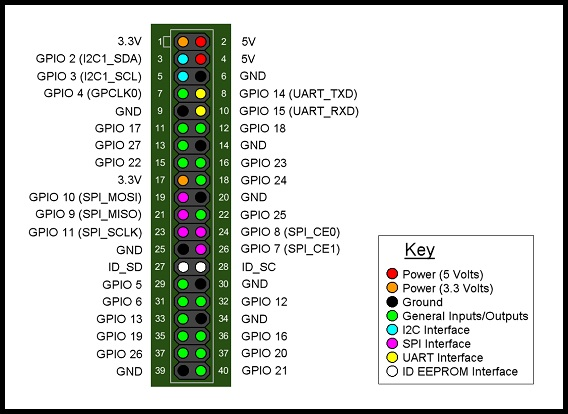
\includegraphics[scale=0.6]{RaspberryPi2_pinout.jpg}
		\centering
		\caption{[4]}
	\end{figure} 
	
	\flushleft
	You must have noticed that the board contains pins named as GPIO (that are used for interfacing input and output devices) and hence in order to refer to the R-Pi pins there exists two modes:
	\begin{enumerate}
		\item \textbf{BCM mode:} Referring the pins with the GPIO number
		\item \textbf{Board mode:} Referring the pins using the IC pin numbers.
	\end{enumerate}
	
	\flushleft
	\newpage
	\section{Experiment}
	 In order to access GPIO pins we need to use the Rpi.GPIO package which is usually present in the Python libraries. (but if you are using an R-Pi 2 please ensure that the version of this package is greater than 0.5.10 )
	 
	 \subsection{Interfacing an LED with R-Pi(BCM mode)}
	 \textbf{Setting up the Hardware}
	 \begin{figure}[h!]
	 	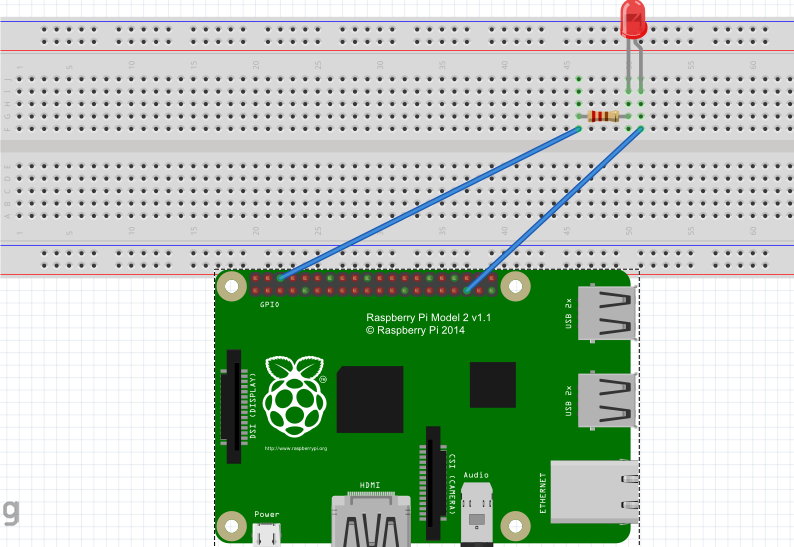
\includegraphics[scale=0.4]{Led.png}
	 	\centering
	 \end{figure}
	 \newline
	 As shown in the figure :
	 \begin{itemize}
	 	\item Anode of the LED is connected to GPIO 19(IC pin 35).
	 	\item Cathode of the LED is connected to a resistor(330 ohms) which is in turn connected to GND pin on R-Pi 2.
	\end{itemize}
		Note: Please refer the theory section for the pin description of R-Pi 2.
	
	\newpage
	\flushleft
	\textbf{Code}
	\lstinputlisting[language=Python]{led_blink_2016.py}
	
	\newpage
	 \subsection{Interfacing a Push button with R-Pi(Board Mode)}
	 \textbf{Setting up Hardware}
	  \begin{figure}[h!]
	  	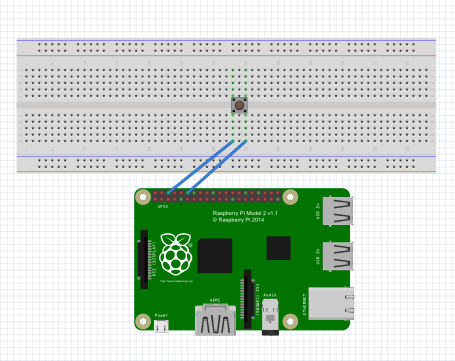
\includegraphics[scale=0.6]{pb.png}
	  	\centering
	  \end{figure}
	   As shown in the figure :
	   \begin{itemize}
	   	\item One pin of the push button is connected to Ground
	   	\item The other pin of the push button is connected to IC pin no. 12
	   \end{itemize}
	    Note: Please refer the theory section for the pin description of R-Pi 2. Also ensure that the push button pins you connect to R-Pi shoudlnt be shorted.
	    \vspace{0.3cm}
	    \newline
	    \textbf{Code}
	    \lstinputlisting[language=Python]{Pushbutton_2016.py}
	 
	 \newpage
	 \subsection{ Controlling an led using a push button.}
	 \textbf{Setting up Hardware}		
		\begin{figure}[h!]
			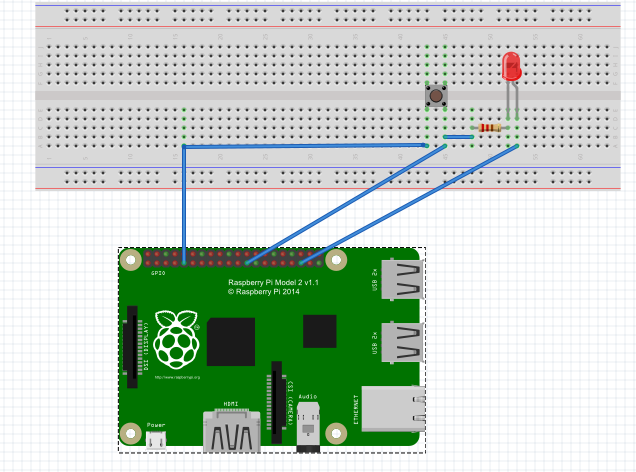
\includegraphics[scale=0.4]{GPIO.png}
			\centering
		\end{figure}
		As shown in figure:
		\begin{itemize}
			\item One pin of the push button is connected to Ground(Pin 9)
			\item The other pin of the push button is connected to IC pin no. 12
			\item The anode of led is connected to IC pin 35 of raspberry pi
			\item The cathode of led is connected to the the resistor of 300 ohms which is then connected to the ground.
		\end{itemize}
		
		Note: Please refer the theory section for the pin description of R-Pi 2. Also ensure that the push button pins you connect to R-Pi should not be shorted.
		\vspace{0.3cm}
		\newline
		\textbf{Code}
		\lstinputlisting[language=Python]{switchpress_LED(GPIO).py}
		
	\section{References}
	\begin{enumerate}
		\item \url{http://www.engadget.com/2012/09/04/raspberry-pi-getting-started-guide-how-to/}
		\item \url{https://www.raspberrypi.org/products/raspberry-pi-2-model-b/}
		\item \url{http://pi4j.com/images/j8header-photo.png}
		\item \url{http://data.designspark.info/uploads/images/53bc258dc6c0425cb44870b50ab30621}
	\end{enumerate}
	
	
\end{document}



